%==============================================================================
%  Final Defense Presentation — PEMFC Modeling and Control
%  Universite Grenoble Alpes — M1 EECS internship
%  Rules: see ../presentation_rules.md  (20 min talk, key equations/results only)
%  Build:  pdflatex main  (run twice)   -> deliver main.pdf
%==============================================================================
\documentclass[aspectratio=169,11pt]{beamer}

% ----------------------------- Theme -----------------------------------------
\usetheme{Madrid}
\usecolortheme{default}
\setbeamertemplate{navigation symbols}{}     % hide nav icons
\setbeamertemplate{caption}[numbered]
\setbeamertemplate{bibliography item}{}

% A clean UGA-style blue
\definecolor{ugablue}{RGB}{0,80,140}
\definecolor{ugagray}{RGB}{90,90,90}
\setbeamercolor{structure}{fg=ugablue}
\setbeamercolor{frametitle}{bg=ugablue,fg=white}
\setbeamercolor{title}{bg=ugablue,fg=white}
\setbeamercolor{subtitle}{bg=ugablue,fg=white}
\setbeamercolor{block title}{bg=ugablue,fg=white}
\setbeamercolor{block body}{bg=ugablue!6,fg=black}
\setbeamerfont{frametitle}{size=\large}
\setbeamertemplate{itemize items}[circle]

% ----------------------------- Packages --------------------------------------
\usepackage[utf8]{inputenc}
\usepackage[T1]{fontenc}
\usepackage{lmodern}
\usepackage[english]{babel}
\usepackage{amsmath,amssymb}
\usepackage{graphicx}
\graphicspath{{figures/}}
\usepackage{booktabs}
\usepackage{tikz}
\usetikzlibrary{arrows.meta,positioning,calc}
\usepackage{pgfplots}
\pgfplotsset{compat=1.16}

% ADDED: small helper to print a source line (bracket numbers match the report)
\newcommand{\srccite}[1]{\par\vspace{2pt}{\scriptsize\color{ugagray}Ref.: #1}}

% ----------------------------- Title data ------------------------------------
\title[PEMFC Modeling and Control]{Modeling and Control of a PEM Fuel Cell Stack}
\subtitle{From physical principles to per-cell calibration and PI-based power control}
\author[K.~E.~Lagha]{Khalil Ellah \textsc{Lagha}}
\institute[UGA / GIPSA-lab]{%
    Universit\'e Grenoble Alpes --- GIPSA-lab, Infinity Team\\[2pt]
    \small Supervisor: Prof.\ Emmanuel \textsc{Witrant}}
\date{M1 EECS Internship Defense --- June 2026}

%==============================================================================
\begin{document}

% ----------------------------- Title -----------------------------------------
{
\setbeamertemplate{footline}{}
\begin{frame}[plain]
    \begin{columns}
        \column{0.5\textwidth}\hfill
\includegraphics[height=1.1cm]{UGAlogo.png}
        \column{0.5\textwidth}
\includegraphics[height=1.1cm]{gipsa-lablogo.jpg}\hfill
    \end{columns}
    \vfill
    \titlepage
    \vfill
\end{frame}
}

% ----------------------------- Outline ---------------------------------------
\begin{frame}{Outline}
    \tableofcontents
    \vfill
    \begin{block}{One-line storyline}
        From an electrochemical model $\rightarrow$ per-cell calibration
        $\rightarrow$ dynamic characterization $\rightarrow$ PI-based power control.
    \end{block}
\end{frame}

%==============================================================================
\section{Motivation \& Objectives}
%==============================================================================

% --- Motivation --------------------------------------------------------------
\begin{frame}{Motivation --- Why Control a PEM Fuel Cell?}
    \begin{columns}[T]
        \column{0.58\textwidth}
        \begin{itemize}
            \item $\mathrm{H_2}\rightarrow$ electricity, only by-products
                  \textbf{water + heat} --- clean transport / stationary power.
            \item PEMFC wins on \textbf{low temperature, high power density,
                  fast start-up}.
            \item Unmanaged operation fails:
                  \begin{itemize}\footnotesize
                      \item reactant starvation $\rightarrow$ irreversible degradation;
                      \item excess anode--cathode pressure $\rightarrow$ membrane damage.
                  \end{itemize}
            \item Cells differ within a stack (deviations up to $\approx 7\%$) ---
                  a stack is \emph{not} one ideal cell.
        \end{itemize}
        \vspace{0.3em}
        \alert{$\Rightarrow$ Feedback control is required --- and it needs a model
        that is simple to analyze yet faithful to the hardware.}
        \srccite{[3] Daud et al.\ 2017; [1] Andrea et al.\ 2006}
        \column{0.42\textwidth}
        \centering
        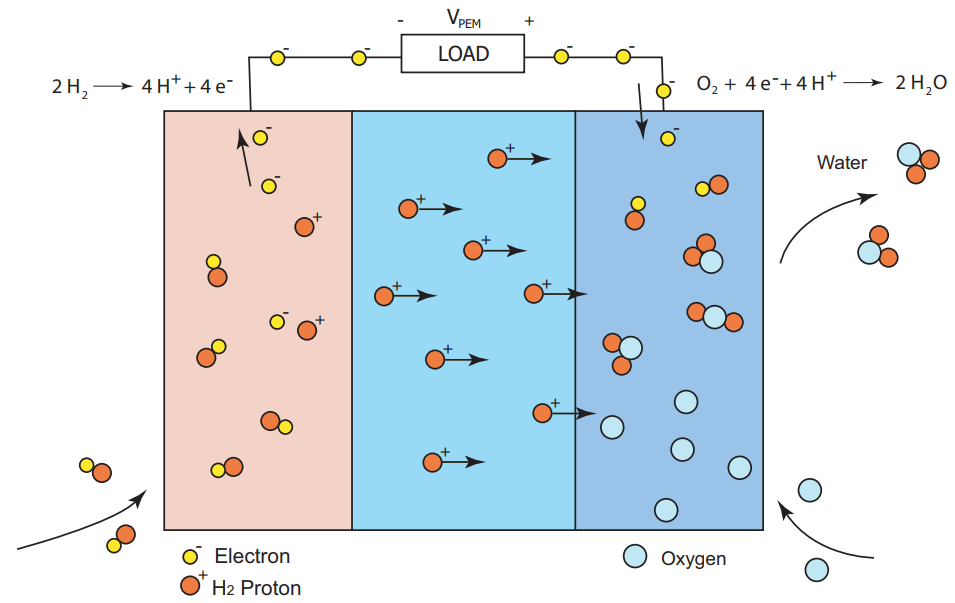
\includegraphics[width=\linewidth]{pemfc_operation.png}\\
        \scriptsize Operating principle of a PEM fuel cell
    \end{columns}
\end{frame}

% --- Objectives --------------------------------------------------------------
\begin{frame}{Internship Objectives}
    \begin{enumerate}
        \item Simplified \textbf{control-oriented dynamic model} of a cell and the
              10-cell stack.
        \item \textbf{Per-cell parameter identification} from bench data.
        \item \textbf{Linearized state-space} model + controllability /
              observability analysis.
        \item \textbf{Experimental} dynamic response to resistive load steps
              (timescales for control bandwidth).
        \item A \textbf{PI-based control architecture} through a DC/DC boost
              converter.
    \end{enumerate}
    \vfill
    \begin{block}{Thread of the talk}
        Each result below maps back to one of these five objectives.
    \end{block}
\end{frame}

%==============================================================================
\section{Experimental Platform}
%==============================================================================

\begin{frame}{Experimental Setup --- The Bench}
    \begin{columns}[T]
        \column{0.6\textwidth}
        \centering
        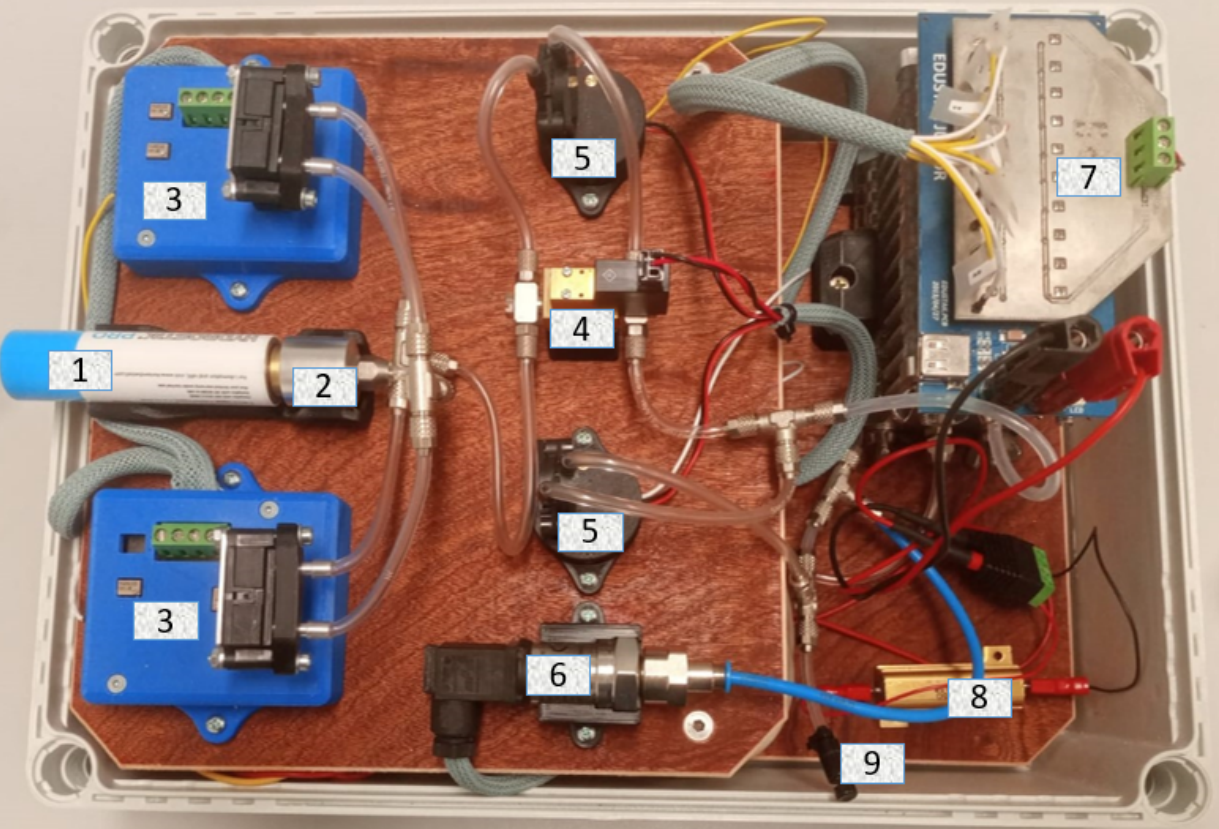
\includegraphics[width=\linewidth]{setup_exp.png}\\
        \scriptsize Instrumented PEMFC bench (numeric call-outs 1--9)
        \column{0.4\textwidth}
        \footnotesize
        \begin{enumerate}
            \item $\mathrm{H_2}$ storage (metal-hydride)
            \item Pressure regulator
            \item Flow sensor (Honeywell AWM42)
            \item Proportional solenoid valve
            \item Pressure sensor (MPX4250DP)
            \item Relative pressure sensor
            \item \textbf{10-cell EDUSTAK JUNIOR stack}
            \item Load resistors ($25 / 3.3 / 6.8\,\Omega$)
            \item Mounting / DAQ base
        \end{enumerate}
    \end{columns}
    \vspace{0.2em}
    \alert{\footnotesize 10-cell stack, per-cell voltage acquisition at 1\,Hz
    via a serial DAQ chain built in the project.}
\end{frame}

%==============================================================================
\section{Background}
%==============================================================================

% --- Operating principle -----------------------------------------------------
\begin{frame}{PEMFC Operating Principle}
    \begin{columns}[T]
        \column{0.56\textwidth}
        \textbf{Half-reactions}
        \begin{itemize}\footnotesize
            \item Anode: $\mathrm{H_2 \rightarrow 2H^+ + 2e^-}$
            \item Cathode: $\mathrm{O_2 + 4H^+ + 4e^- \rightarrow 2H_2O}$
            \item Overall:
                  $\mathrm{H_2 + \tfrac12 O_2 \rightarrow H_2O}$ + electricity + heat
        \end{itemize}
        \vspace{0.3em}
        \begin{itemize}
            \item Protons cross the membrane; electrons drive the load.
            \item MEA = elementary repeating unit of the stack.
            \item \textbf{Water management is critical}: dry $\rightarrow$ low
                  conductivity, flooded $\rightarrow$ blocked channels.
        \end{itemize}
        \srccite{[9] Pukrushpan 2003}
        \column{0.44\textwidth}
        \centering
        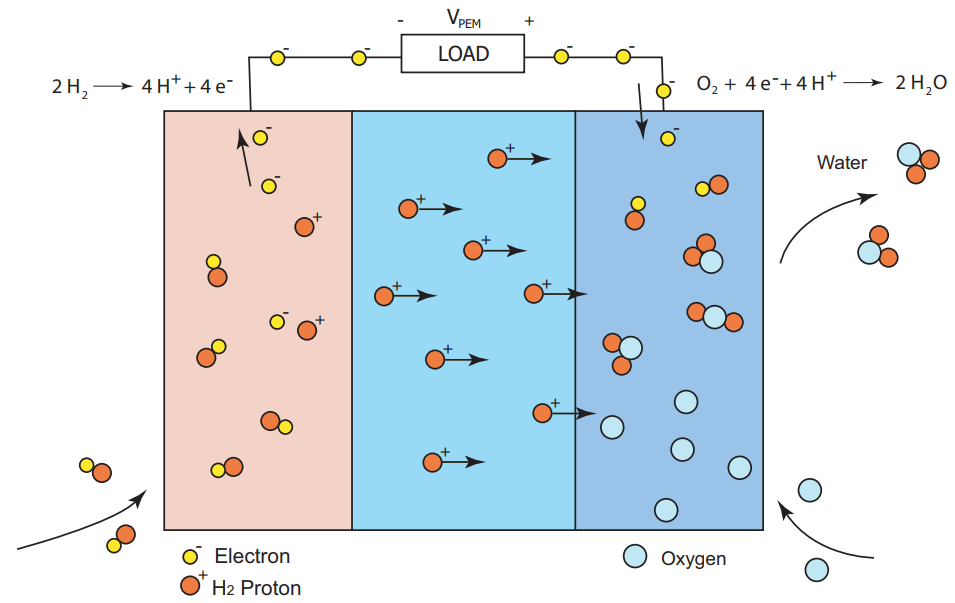
\includegraphics[width=\linewidth]{pemfc_operation.png}\\
        \scriptsize Charge transport in a single cell
    \end{columns}
\end{frame}

% --- Losses ------------------------------------------------------------------
\begin{frame}{Voltage Losses \& Polarization Curve}
    \begin{columns}[T]
        \column{0.5\textwidth}
        Three loss regimes shape the curve:
        \begin{itemize}
            \item \textbf{Activation} --- low current (reaction kinetics)
            \item \textbf{Ohmic} --- mid range ($\approx$ linear)
            \item \textbf{Concentration} --- high current (mass transport)
        \end{itemize}
        \vspace{0.3em}
        \alert{The polarization curve = cell voltage vs.\ current density = the
        backbone of the model.}
        \srccite{[1] Andrea et al.\ 2006}
        \column{0.5\textwidth}
        \centering
        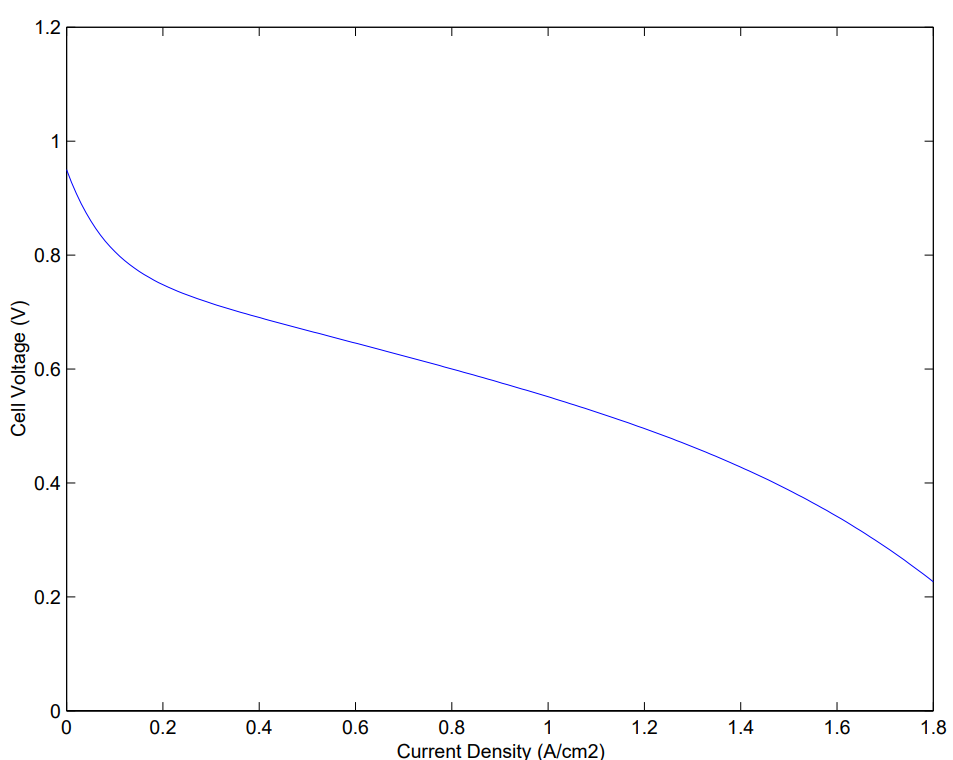
\includegraphics[width=\linewidth]{pemfc_polarization_curve.png}\\
        \scriptsize Polarization curve (losses bend the ideal flat voltage)
    \end{columns}
\end{frame}

% --- Practical challenge -> control choice -----------------------------------
\begin{frame}{Practical Challenge $\rightarrow$ Control-Strategy Choice}
    \begin{itemize}
        \item Natural actuator = \textbf{hydrogen supply}, but usable pressure is
              \textbf{narrowly bounded} (regulator cap + membrane-damage risk).
        \item The valve \textbf{saturates} before meeting the load demand
              $\rightarrow$ too little authority for direct current control.
    \end{itemize}
    \vspace{0.3em}
    \begin{block}{Decision}
        \alert{Move control to the electrical side:}
        stack $\rightarrow$ \textbf{DC/DC boost converter} $\rightarrow$ fast
        \textbf{PI loop}.
    \end{block}
    \centering\footnotesize
    Roles: \emph{electrical control for the fast dynamics, gas supply for the
    slow operating conditions.}
    \srccite{[16] Zhu et al.\ 2017; [6] Kharrat \& Haußmann 2025}
\end{frame}

%==============================================================================
\section{Simplified Model}
%==============================================================================

% --- Architecture ------------------------------------------------------------
\begin{frame}{Model Architecture}
    \centering
    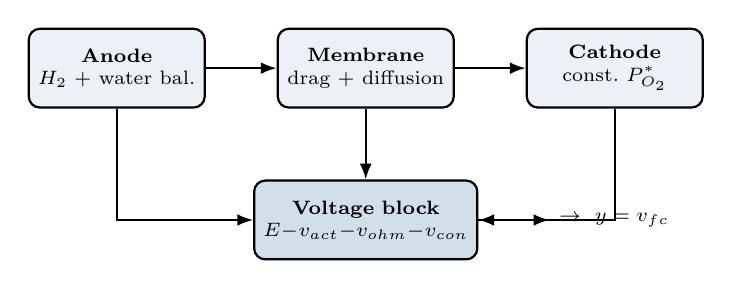
\begin{tikzpicture}[
        >=Latex, font=\scriptsize,
        blk/.style={draw, thick, rounded corners, fill=ugablue!8, align=center,
            minimum height=1.0cm, text width=2.0cm},
        vb/.style={draw, thick, rounded corners, fill=ugablue!18, align=center,
            minimum height=1.0cm, text width=2.6cm},
        line/.style={-{Latex[length=2mm]}, thick}]
        \node[blk] (an) {\textbf{Anode}\\ $H_2$ + water bal.};
        \node[blk, right=0.9cm of an] (mb) {\textbf{Membrane}\\ drag + diffusion};
        \node[blk, right=0.9cm of mb] (ca) {\textbf{Cathode}\\ const.\ $P_{O_2}^{*}$};
        \node[vb, below=0.9cm of mb] (vb) {\textbf{Voltage block}\\ $E-v_{act}-v_{ohm}-v_{con}$};
        \node[right=0.9cm of vb, align=center] (out) {$\rightarrow\ y=v_{fc}$};
        \draw[line] (an) -- (mb);  \draw[line] (mb) -- (ca);
        \draw[line] (an.south) |- (vb.west);
        \draw[line] (mb) -- (vb);
        \draw[line] (ca.south) |- (vb.east);
        \draw[line] (vb) -- (out);
    \end{tikzpicture}

    \vspace{0.3em}
    \begin{columns}[T]
        \column{0.5\textwidth}
        \footnotesize\textbf{States / inputs / output}
        \begin{itemize}\footnotesize
            \item $x=(P_{H_2},\,m_{w,an},\,m_{w,ca})$
            \item $u=(i_{FC}\,[\text{dist.}],\,W_{H_2,in}\,[\text{man.}])$, $y=v_{fc}$
        \end{itemize}
        \column{0.5\textwidth}
        \footnotesize\textbf{Assumptions}
        \begin{itemize}\footnotesize
            \item $H_2$ + air only; ideal gas; slow $T$
            \item $P_{O_2}^{*}=0.21\,P_{atm}$ fixed
        \end{itemize}
    \end{columns}
    \srccite{[9] Pukrushpan 2003; [11] Thanapalan et al.\ 2008}
\end{frame}

% --- Voltage equations -------------------------------------------------------
\begin{frame}{Voltage Equations (6 Parameters per Cell)}
    \textbf{Open-circuit (Nernst) potential:}
    \begin{equation*}
        E = 1.229 - 0.85\!\times\!10^{-3}(T_{fc}-298.15)
        + 4.31\!\times\!10^{-5}\,T_{fc}\!\left(\ln p_{H_2} + \tfrac12\ln p_{O_2}\right)
    \end{equation*}
    \textbf{Cell voltage} = reversible voltage $-$ three semi-empirical losses:
    \begin{equation*}
        v_{fc} = E - \underbrace{v_{act}}_{\text{activation}}
                   - \underbrace{v_{ohm}}_{\text{ohmic}}
                   - \underbrace{v_{con}}_{\text{concentration}}
    \end{equation*}
    \begin{block}{Calibrated unknowns}
        \alert{Six parameters per cell} $\theta=(\xi_1,\xi_2,\xi_3,\xi_4,B,c)$;
        stack voltage $V_s=\sum_{\text{cells}} v_{fc}$.
    \end{block}
    \srccite{[11] Thanapalan et al.\ 2008; [2] Cao et al.\ 2019 --- full derivation in backup}
\end{frame}

% --- Dynamic equations -------------------------------------------------------
\begin{frame}{Dynamic Equations}
    \textbf{Anode (hydrogen pressure):}
    \begin{equation*}
        \dot P_{H_2}=\frac{R_{H_2}T}{V_{an}}
        \left(W_{H_2,in}-W_{H_2,out}-\frac{M_{H_2}n}{2F}\,i_{FC}\right)
    \end{equation*}
    \begin{itemize}
        \item \textbf{Membrane:} electro-osmotic drag + back-diffusion;
              Springer sorption isotherm $\lambda(a)$.
        \item \textbf{Cathode:} constant $P_{O_2}^{*}$; water balance with
              reaction-generated water.
    \end{itemize}
    \vspace{0.2em}
    \begin{block}{Simplifications (cost of being control-oriented)}
        \footnotesize No spatial gradients, no oxygen transient, no liquid water
        $\rightarrow$ low order, fast to simulate and linearize.
    \end{block}
    \srccite{[14] Weber \& Newman 2004; [15] Zhang et al.\ 2017}
\end{frame}

%==============================================================================
\section{Identification \& Analysis}
%==============================================================================

% --- Identification ----------------------------------------------------------
\begin{frame}{Per-Cell Parameter Identification --- DE Convergence}
    \centering
    
\includegraphics[width=0.98\textwidth]{cost_evolution_exp19.png}\\[3pt]
    {\scriptsize RMSE vs.\ generation (log scale) for the 10 cells; dashed line =
    final RMSE after L-BFGS-B refinement. Most cells converge in a few tens of
    generations.}
\end{frame}

\begin{frame}{Per-Cell Parameter Identification --- Method}
    \textbf{Goal:} fit the six parameters
    $\theta=(\xi_1,\xi_2,\xi_3,\xi_4,B,c)$ of each cell.
    \begin{itemize}
        \item Minimize \textbf{RMSE} between model and measured cell voltage over a
              calibration window.
        \item Two-stage optimizer: \emph{differential evolution} (global; pop.\ 20,
              $\le$800 gen., fixed seed) $\rightarrow$ \emph{L-BFGS-B} (local
              refinement).
        \item Bounds encode physics: $\xi_4\le0$, $B\ge0$, $c\ge0$.
    \end{itemize}
    \vfill
    \alert{Final per-cell RMSE: 2.0--11.3\,mV for the healthy cells
    (mean 8.0\,mV).}
    \srccite{[2] Cao et al.\ 2019; [11] Thanapalan et al.\ 2008}
\end{frame}

% --- State-space -------------------------------------------------------------
\begin{frame}{Linearized State-Space Model}
    \[
        \dot{\mathbf{x}}=A\mathbf{x}+B\mathbf{u},\qquad y=C\mathbf{x}+D\mathbf{u},
        \qquad
        \mathbf{x}=\!\begin{bmatrix}P_{H_2}\\ m_{w,an}\\ m_{w,ca}\end{bmatrix}\!,\;
        \mathbf{u}=\!\begin{bmatrix}i_{FC}\\ W_{H_2,in}\end{bmatrix}
    \]
    \begin{columns}[T]
        \column{0.46\textwidth}
        \begin{block}{$A,B$ --- read off directly}
            \footnotesize Hydrogen-pressure + two water balances are
            \emph{linear} at constant $T$.
        \end{block}
        \column{0.54\textwidth}
        \begin{block}{$C,D$ --- Jacobian linearization}
            \footnotesize Voltage output is \emph{nonlinear} (logs of
            $P_{H_2},i_{FC}$; membrane resistivity) $\Rightarrow$ first-order
            Taylor expansion.
        \end{block}
    \end{columns}
    \vspace{0.3em}
    \[
    A=\begin{bmatrix}0&0&0\\ 0&-\beta&\gamma\\ 0&\beta&-\gamma\end{bmatrix},\qquad
    B=\begin{bmatrix}
        -\tfrac{R_{H_2}T M_{H_2} n}{2F V_{an}} & \tfrac{R_{H_2}T}{V_{an}}\\
        d_1 & 0\\ d_2 & 0
    \end{bmatrix}
    \]
\end{frame}

% --- Controllability / Observability -----------------------------------------
\begin{frame}{Controllability \& Observability}
    \begin{block}{Controllability}
        \alert{Controllable} for all physically realistic electro-osmotic drag
        coefficients $n_d$ (singular only at one degenerate condition
        $n_d=\tfrac{nV_{an}}{2(V_{an}+V_{ca})}$).
    \end{block}
    \begin{block}{Observability (voltage-only output)}
        Voltage \alert{observes $P_{H_2}$ but not the water states}
        $\Rightarrow$ a \textbf{reduced-order voltage-based observer} suffices for
        hydrogen-pressure regulation; full-state would need extra sensors.
    \end{block}
    \vfill
    \centering\footnotesize
    Consequence: a voltage measurement is enough to track the pressure state we
    actually want to regulate.
\end{frame}

%==============================================================================
\section{Experiments \& Results}
%==============================================================================

% --- Protocols ---------------------------------------------------------------
\begin{frame}{Experimental Protocols}
    \begin{itemize}
        \item 10-cell stack; per-cell voltage at \textbf{1\,Hz} via the project's
              serial DAQ chain.
        \item \textbf{Optimization Experiment} (Apr 2026): $25\,\Omega$ connected
              at $t=135$\,s, removed at $t=684$\,s $\rightarrow$ calibration data.
        \item \textbf{TR-current steps} (9 Jun 2026): $3.3\,\Omega$ and
              $6.8\,\Omega$ from open circuit; fit
              $I(t)=I_{ss}+\Delta I\,e^{-t/\tau_I}$.
    \end{itemize}
    \vfill
    \begin{block}{Two experiments, two purposes}
        Optimization Experiment $\rightarrow$ \emph{static} calibration;
        TR-current steps $\rightarrow$ \emph{dynamic} timescales for control.
    \end{block}
\end{frame}

% --- Result: stack voltage & current -----------------------------------------
\begin{frame}{Result --- Stack Voltage \& Load Current}
    \centering
    
\includegraphics[width=0.72\textwidth]{comparison_exp19_stack.png}
    \vspace{0.2em}
    \begin{itemize}\footnotesize
        \item OCV $\approx \mathbf{4.57}$\,V $\rightarrow \approx 0.8$\,V under the
              $25\,\Omega$ load; simulation \textbf{tracks} the measurement across
              the loaded window.
        \item \alert{Per-cell fits aggregate correctly to the stack level.}
    \end{itemize}
\end{frame}

% --- Result: V-I fits --------------------------------------------------------
\begin{frame}{Result --- Per-Cell V--I Calibration Fits}
    \centering
    
\includegraphics[width=0.98\textwidth]{all_cells_overview_exp19.png}\\[3pt]
    {\scriptsize Measured points (blue) vs.\ identified model (red), all 10 cells.
    Per-cell calibration RMSE in each panel title.}
\end{frame}

\begin{frame}{Result --- V--I Fits: Findings}
    \begin{itemize}
        \item Healthy cells matched with calibration RMSE \textbf{2.0--11.3\,mV}
              (all below 12\,mV).
        \item Concentration ($B$) and contact-resistance ($c$) terms stay
              $\approx 0$.
        \item[$\Rightarrow$] \alert{Activation and ohmic effects dominate} the
              covered operating range.
        \item Six parameters per cell are enough to reproduce each healthy cell.
    \end{itemize}
\end{frame}

% --- Result: time series -----------------------------------------------------
\begin{frame}{Result --- Per-Cell Voltage: Measured vs.\ Simulated}
    \centering
    
\includegraphics[width=0.98\textwidth]{comparison_exp19_cells.png}\\[3pt]
    {\scriptsize Measured (blue) vs.\ simulated (red) over the full experiment,
    all 10 cells. Per-cell time-series RMSE in each panel title.}
\end{frame}

\begin{frame}{Result --- Time-Series Fit: Findings}
    \begin{itemize}
        \item Healthy cells (3--9) tracked closely across the loaded window.
        \item \textbf{Mean time-series RMSE = 8.0\,mV} for the healthy cells.
        \item Cells 0--2 stay near zero under load $\rightarrow$ degraded
              (next slide).
        \item Larger residuals on Cells 7 and 9 come from the load-on transient,
              excluded from the calibration window.
    \end{itemize}
\end{frame}

% --- Result: diagnosis -------------------------------------------------------
\begin{frame}{Result --- Identification Doubles as Diagnosis}
    \begin{itemize}
        \item \alert{Cells 0, 1, 2 collapse to $\approx 0$\,V} under load
              (top-left panels of the previous figure).
        \item The optimizer returns \textbf{identical, degenerate} parameter sets
              for them (RMSE $<0.1$\,mV against a flat signal).
        \item This is a \textbf{dead-electrode signature}, not a physically
              meaningful fit --- no parameters within the bounds can reproduce a
              dead cell.
    \end{itemize}
    \vfill
    \begin{block}{Takeaway}
        \footnotesize The calibration is also a \textbf{health check}: it flags
        faulty cells automatically. Full per-cell parameter table in
        \textbf{backup~B2}.
    \end{block}
\end{frame}

% --- Result: load-step raw channels [if time] --------------------------------
\begin{frame}{Result --- Load-Step Raw Channels: $R=3.3\,\Omega$ \hfill {\small[if time]}}
    \begin{columns}[c]
        \column{0.6\textwidth}
        \centering
        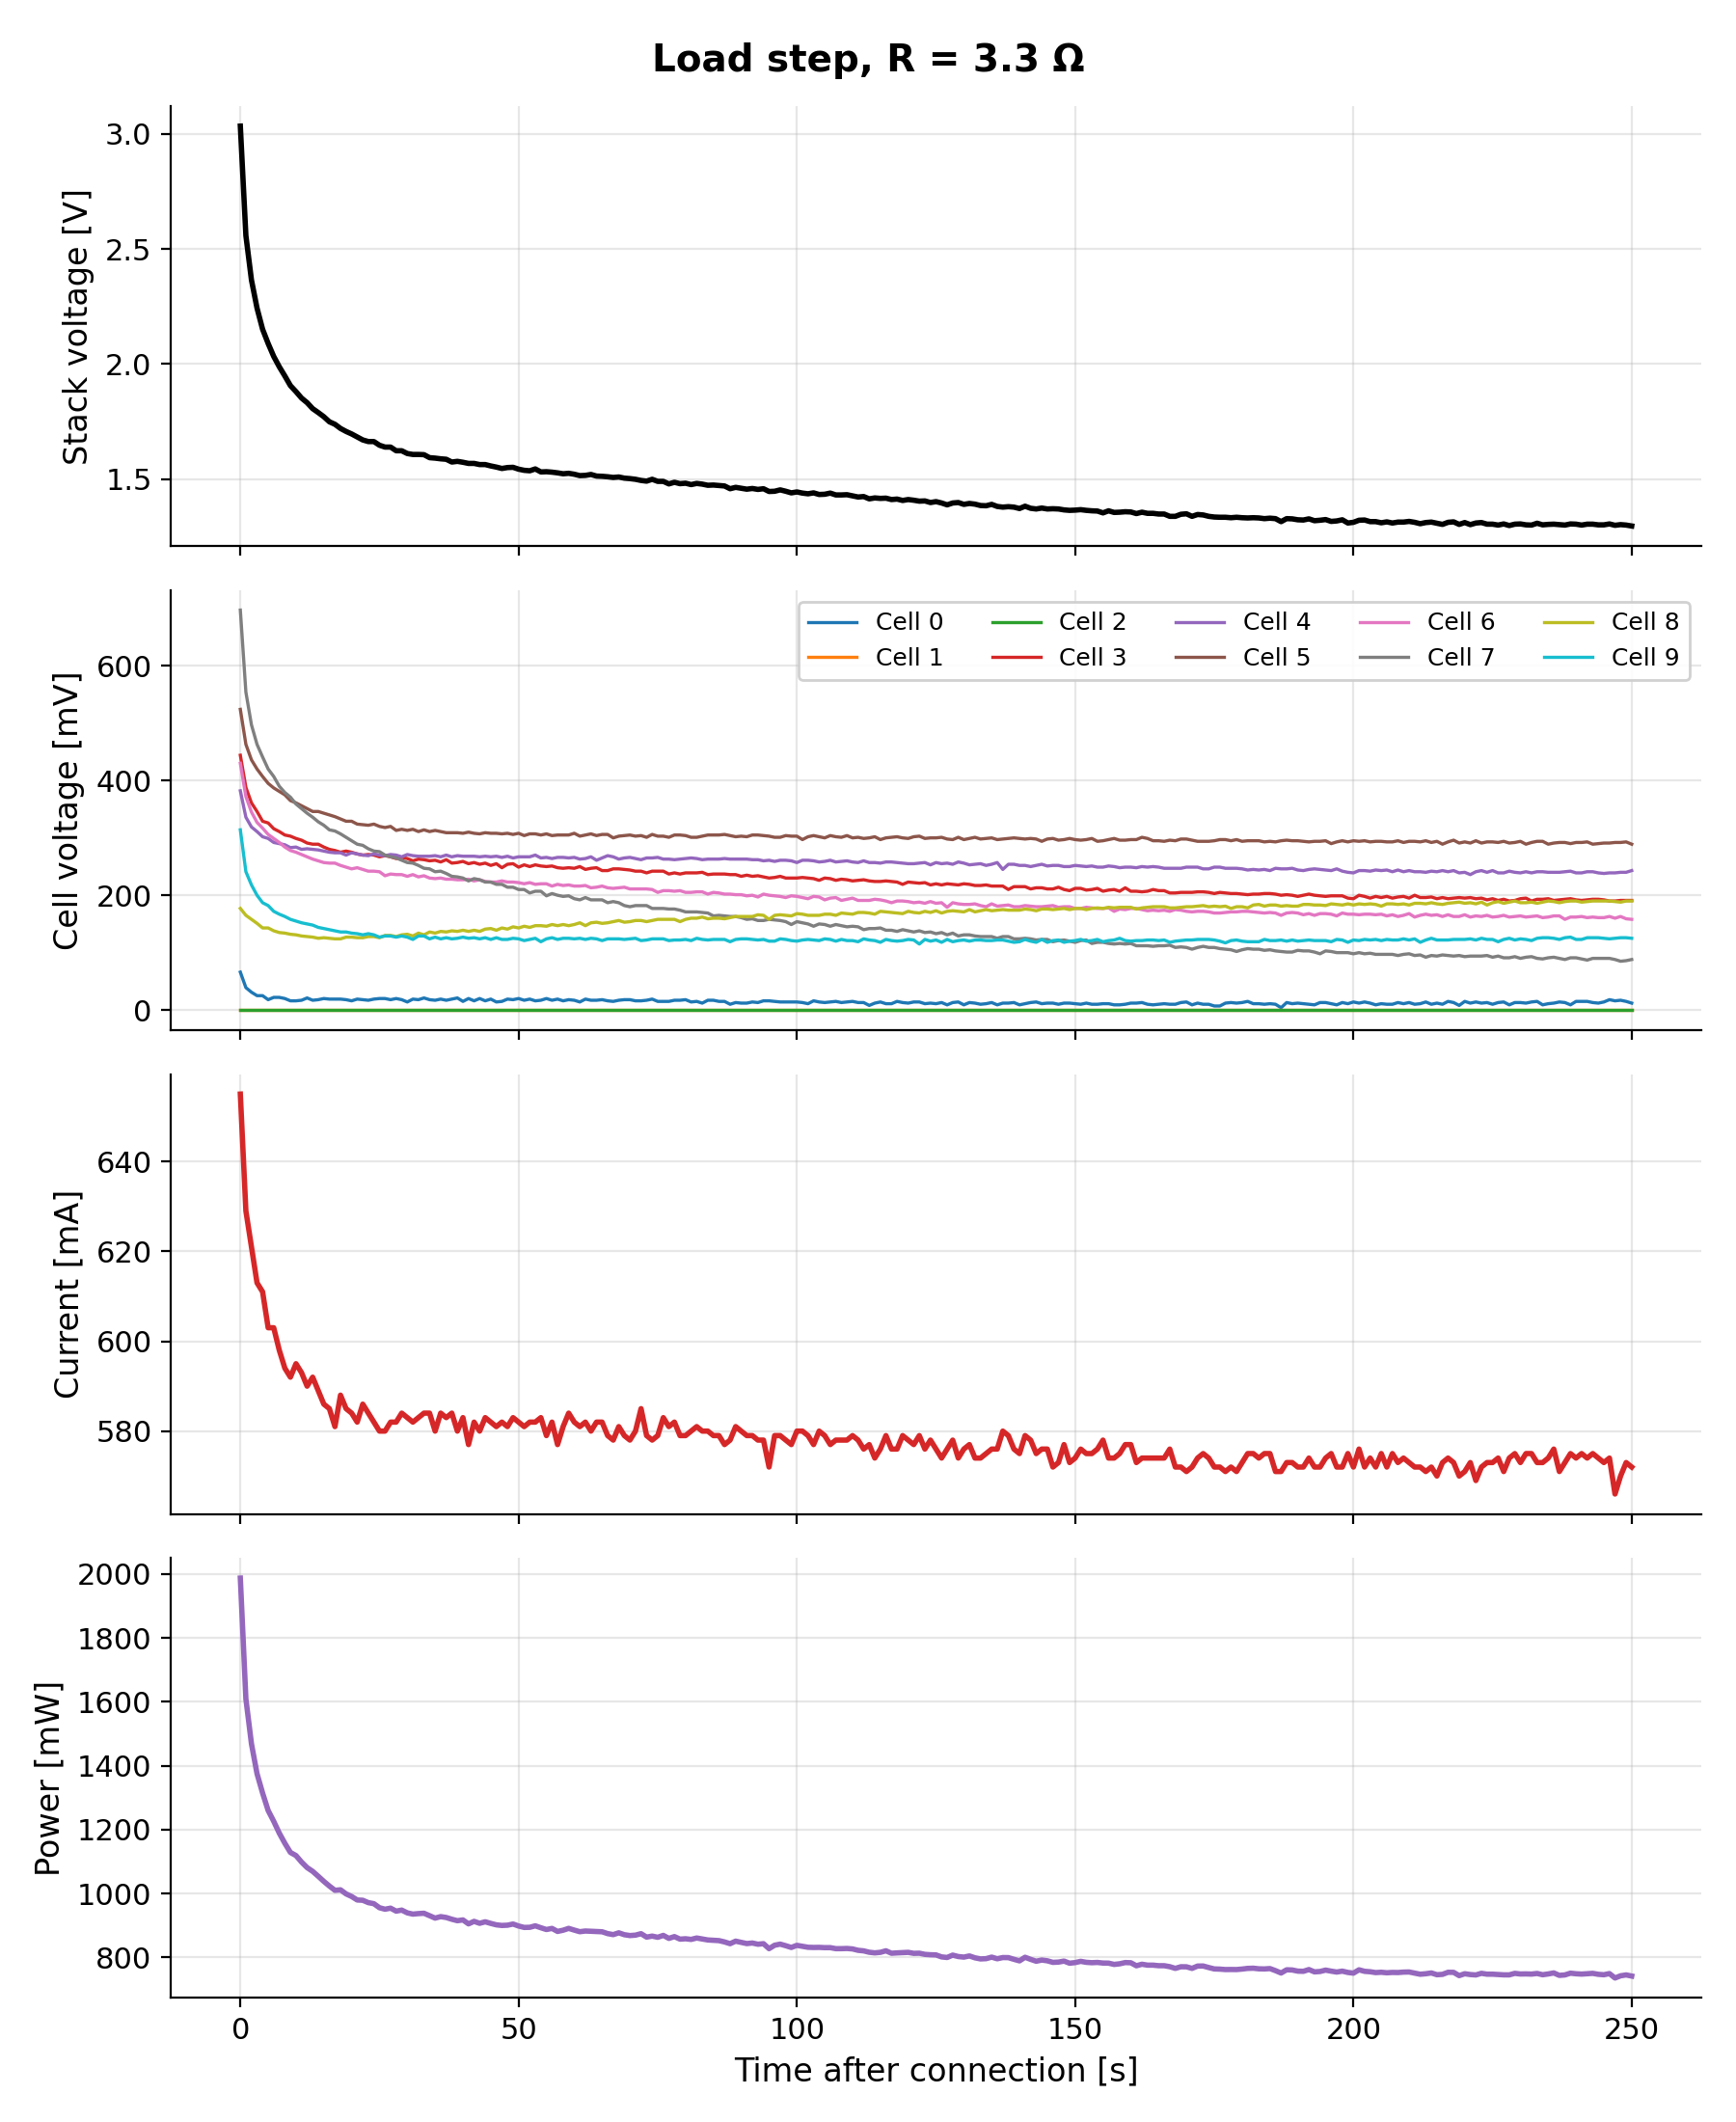
\includegraphics[height=0.85\textheight]{exp_33ohm_plot.png}
        \column{0.4\textwidth}
        \footnotesize
        Four channels after the step: stack voltage, individual cell voltages,
        current, and power.
        \vspace{0.8em}

        \alert{Monotonic relaxation, no overshoot $\Rightarrow$ first-order
        behavior.}
    \end{columns}
\end{frame}

\begin{frame}{Result --- Load-Step Raw Channels: $R=6.8\,\Omega$ \hfill {\small[if time]}}
    \begin{columns}[c]
        \column{0.6\textwidth}
        \centering
        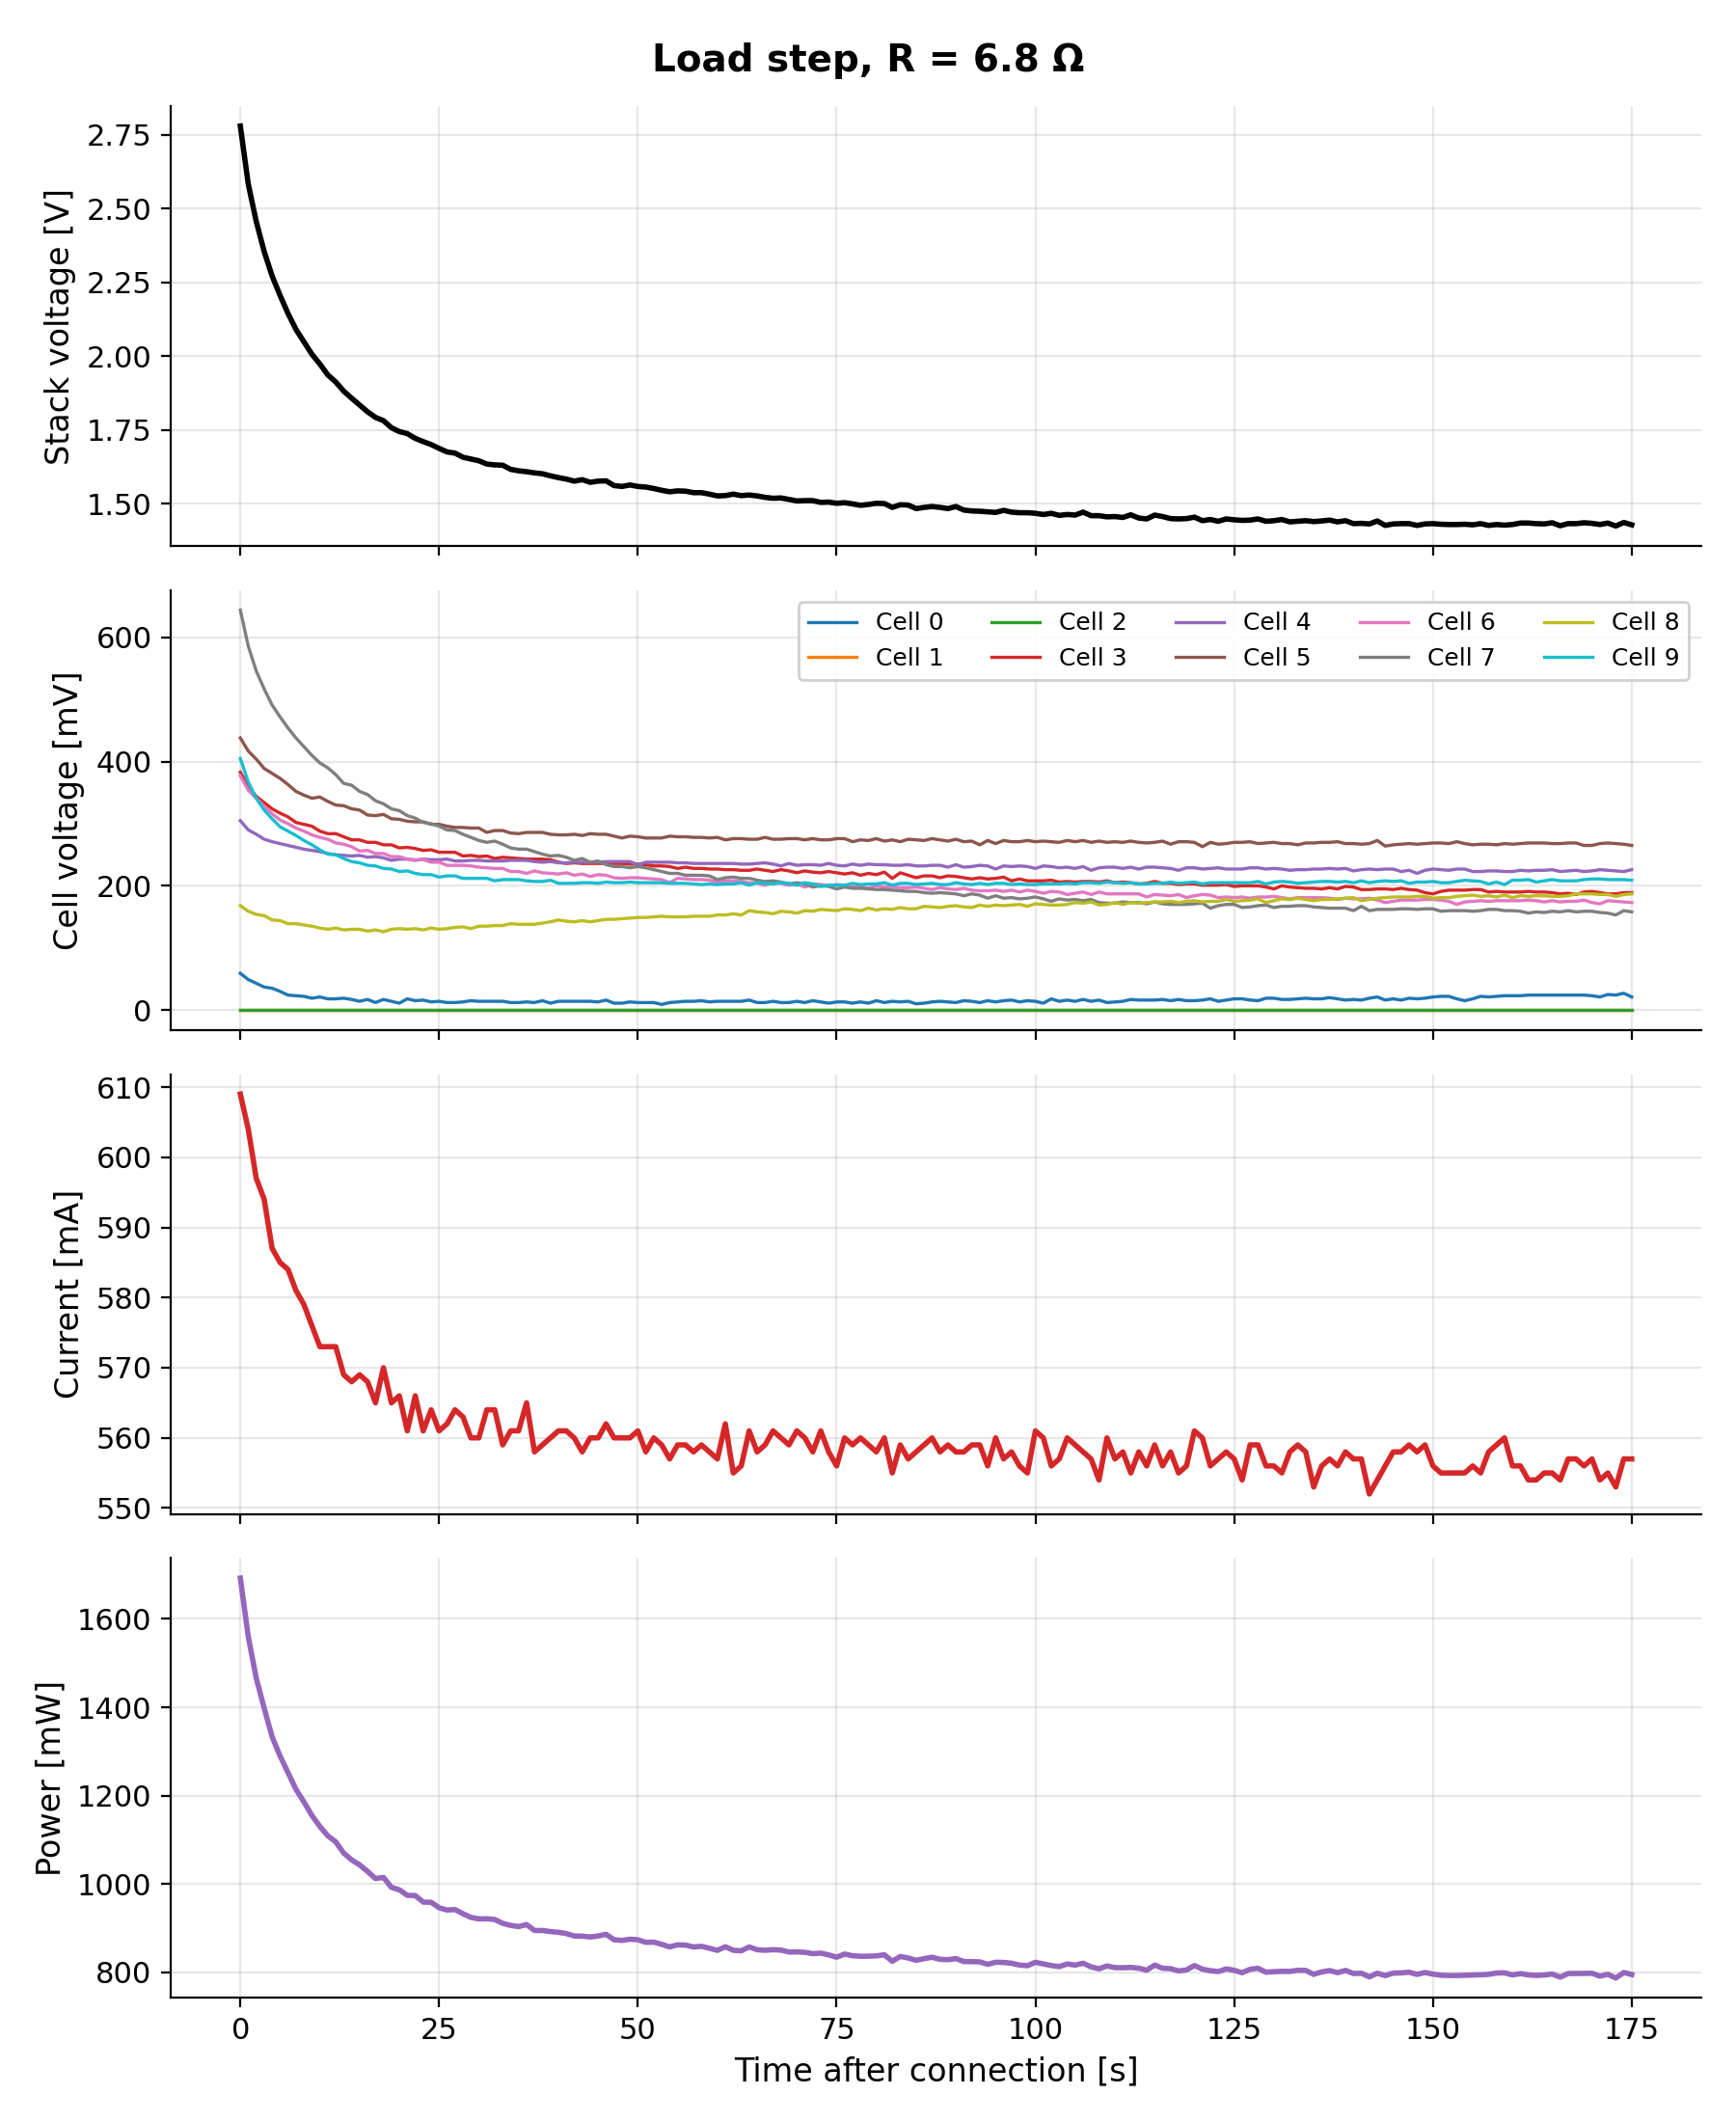
\includegraphics[height=0.85\textheight]{exp_68ohm_plot.png}
        \column{0.4\textwidth}
        \footnotesize
        Same four channels under the lighter load. The current settles more
        slowly than at $3.3\,\Omega$.
        \vspace{0.8em}

        \alert{Same first-order shape, longer time constant.}
    \end{columns}
\end{frame}

% --- Result: step fit & time constants ---------------------------------------
\begin{frame}{Result --- Current Step Response \& Time Constants}
    \centering
    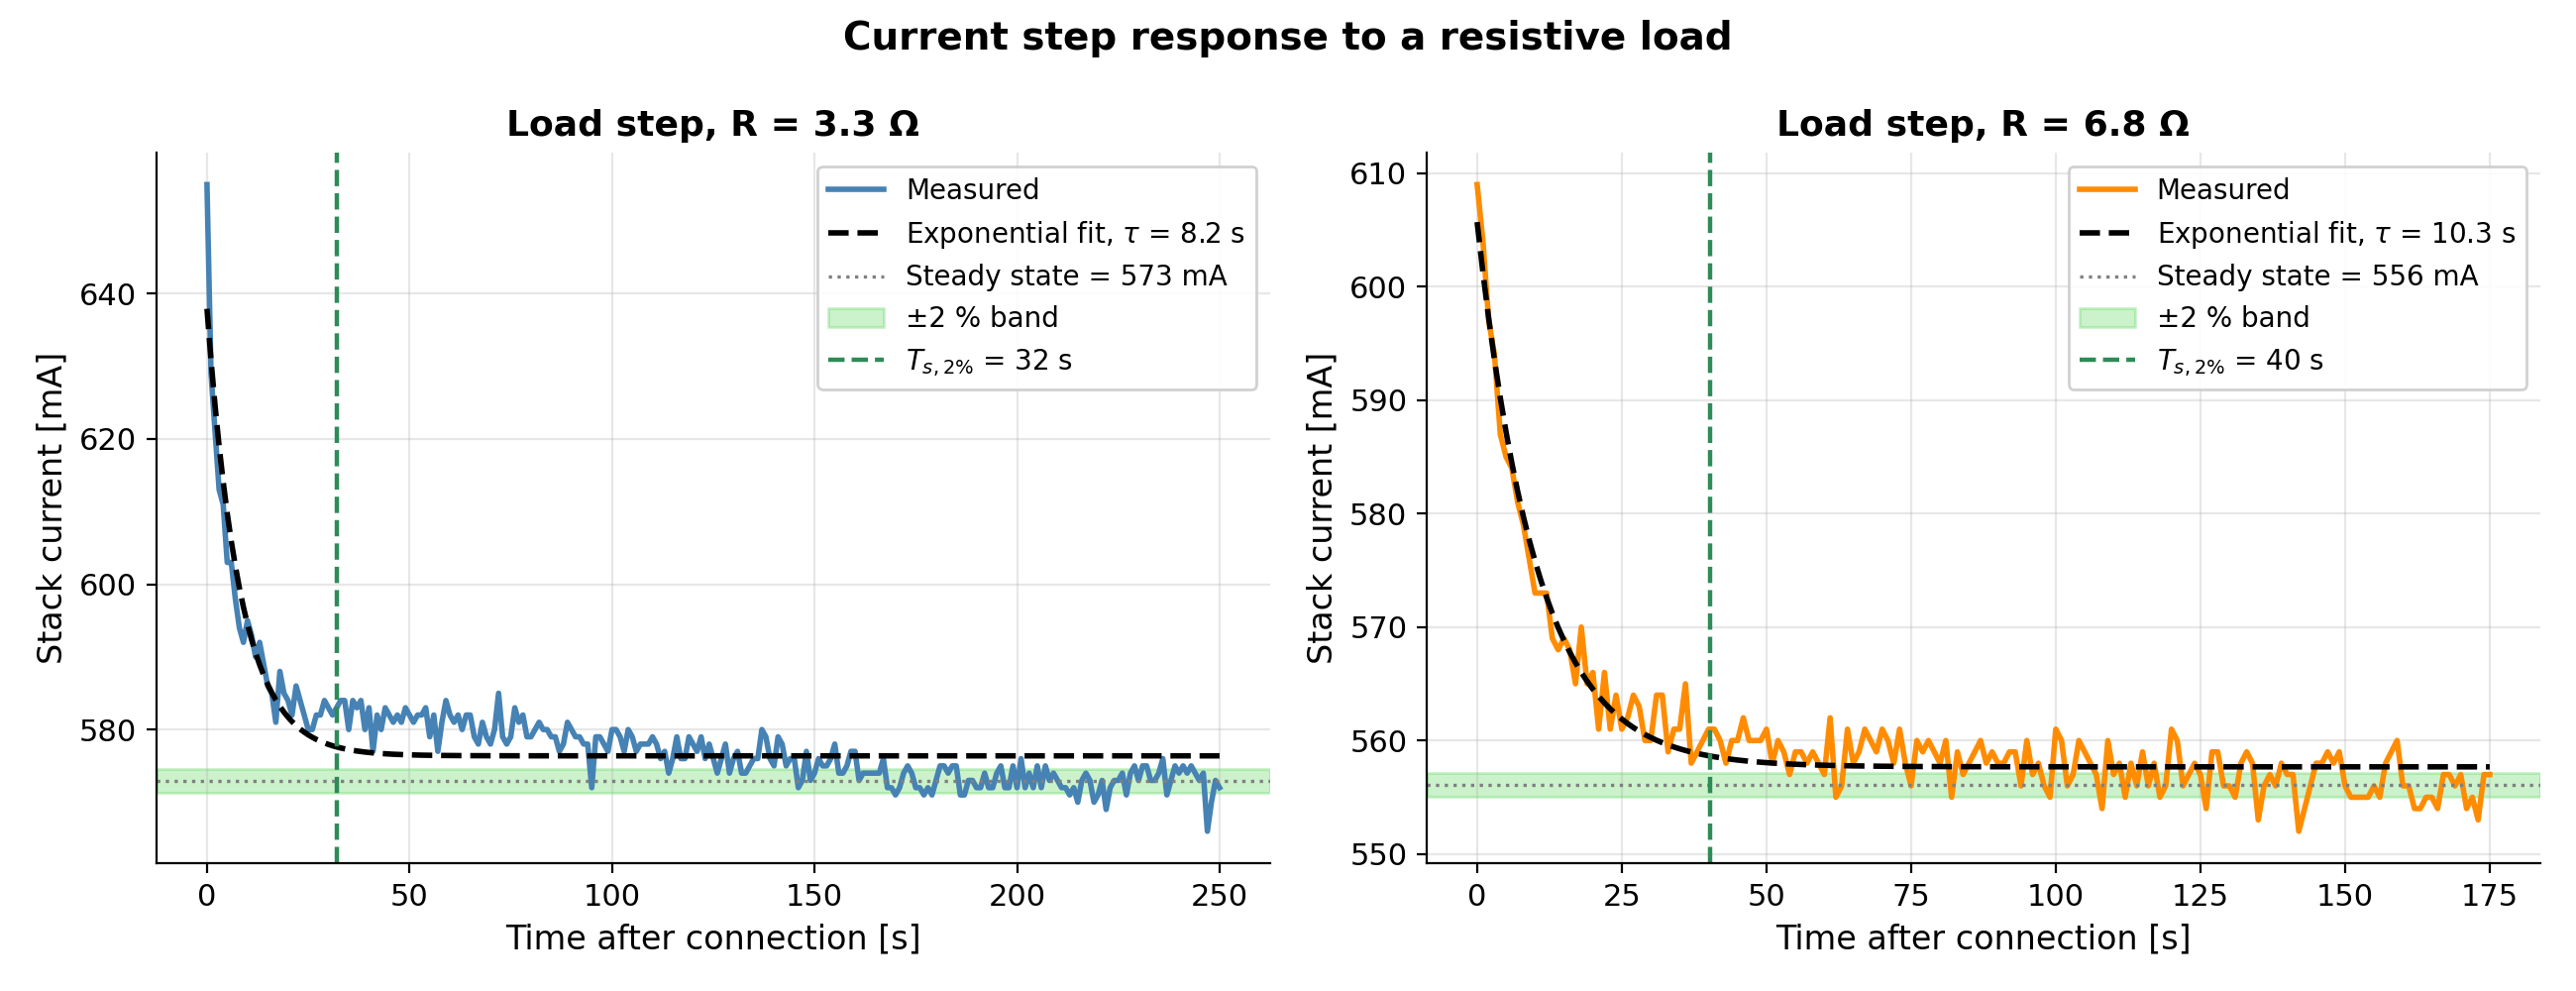
\includegraphics[width=0.92\textwidth]{response_time_plot.png}
    \vspace{0.2em}
    \begin{columns}[T]
        \column{0.42\textwidth}
        \centering\footnotesize
        \begin{tabular}{lcc}
            \toprule
            & $3.3\,\Omega$ & $6.8\,\Omega$ \\
            \midrule
            $\tau_I$ [s]        & 8.2  & 10.3 \\
            $\Delta I$ [mA]     & 82.1 & 52.9 \\
            $T_{s,2\%}$ [s]     & 32.0 & 40.2 \\
            \bottomrule
        \end{tabular}
        \column{0.58\textwidth}
        \footnotesize
        \begin{itemize}
            \item Lighter load $\Rightarrow$ slower (lower current density).
            \item \alert{Control target: act well within $\tau_I\approx 8$--$10$\,s.}
        \end{itemize}
    \end{columns}
\end{frame}

%==============================================================================
\section{Control Architecture}
%==============================================================================

% --- Boost + PI architecture -------------------------------------------------
\begin{frame}{DC/DC Boost Converter + PI Controller}
    \centering
    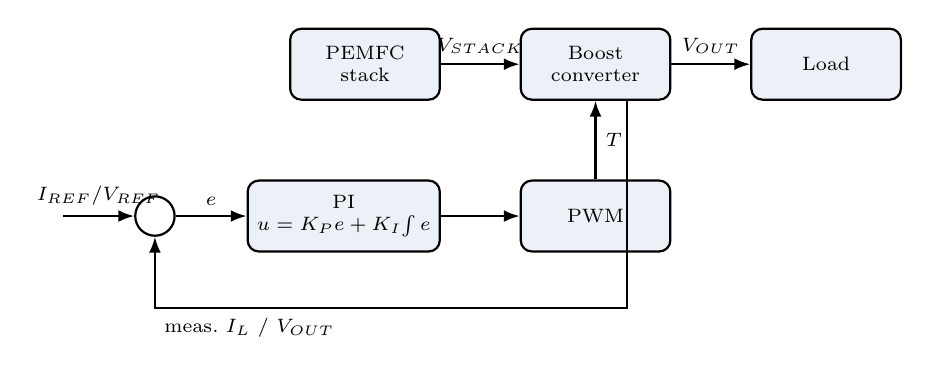
\begin{tikzpicture}[
        >=Latex, font=\scriptsize,
        blk/.style={draw, thick, rounded corners, fill=ugablue!8, align=center,
            minimum height=0.9cm, minimum width=1.9cm},
        sum/.style={draw, thick, circle, minimum size=0.5cm, inner sep=0pt},
        line/.style={-{Latex[length=2mm]}, thick}]
        \node[blk] (fc) {PEMFC\\ stack};
        \node[blk, right=1.0cm of fc] (bo) {Boost\\ converter};
        \node[blk, right=1.0cm of bo] (ld) {Load};
        \node[blk, below=1.0cm of bo] (pwm) {PWM};
        \node[blk, left=1.0cm of pwm] (pi) {PI\\ $u=K_Pe+K_I\!\int e$};
        \node[sum, left=0.9cm of pi] (s) {};
        \draw[line] (fc) -- node[above]{$V_{STACK}$} (bo);
        \draw[line] (bo) -- node[above]{$V_{OUT}$} (ld);
        \draw[line] (pwm) -- node[right]{$T$} (bo);
        \draw[line] (pi) -- (pwm);
        \draw[line] (s) -- node[above]{$e$} (pi);
        \draw[line] ([xshift=-0.9cm]s.west) -- node[above]{$I_{REF}/V_{REF}$} (s);
        \draw[line] ([xshift=0.4cm]bo.south) |- ([yshift=-0.7cm]pi.south)
            -| node[pos=0.25,below]{meas.\ $I_L$ / $V_{OUT}$} (s);
    \end{tikzpicture}
    \vspace{0.2em}
    \begin{block}{Key idea}
        \footnotesize The stack is \emph{neither} an ideal current nor voltage
        source --- the \alert{regulated converter output} is shaped into one by
        the PI loop on the duty cycle $T$.
    \end{block}
    \srccite{[4] Derbeli et al.\ 2017; [16] Zhu et al.\ 2017}
\end{frame}

% --- Current vs voltage source -----------------------------------------------
\begin{frame}{Current-Source vs.\ Voltage-Source Operation}
    \begin{columns}[T]
        \column{0.5\textwidth}
        \begin{block}{Current mode (protect the stack)}
            \footnotesize
            \begin{itemize}
                \item Regulate $I_L \rightarrow I_{REF}$; $e=I_{REF}-I_L$.
                \item $I_{REF}=9.74$\,A = max-power point (50\,W stack; 10\,A hard
                      limit).
                \item Prevents \textbf{overcurrent}.
            \end{itemize}
        \end{block}
        \column{0.5\textwidth}
        \begin{block}{Voltage mode (fixed load voltage)}
            \footnotesize
            \begin{itemize}
                \item Regulate $V_{OUT} \rightarrow V_{REF}$; $e=V_{REF}-V_{OUT}$.
                \item Same averaged converter model.
                \item Natural for \textbf{output-voltage} supply.
            \end{itemize}
        \end{block}
    \end{columns}
    \vspace{0.3em}
    \centering\footnotesize
    Same PI structure \& converter model --- differ only in the feedback variable.
    Online (Ziegler--Nichols-style) tuning, no plant transfer function needed.
    \srccite{[4] Derbeli et al.\ 2017}
\end{frame}

%==============================================================================
\section{Conclusion}
%==============================================================================

% --- Conclusion --------------------------------------------------------------
\begin{frame}{Conclusion}
    \begin{itemize}
        \item Six-parameter model fitting all healthy cells \textbf{$<12$\,mV};
              built-in \textbf{diagnosis} of degraded cells (0,1,2).
        \item Explicit \textbf{state-space} model: controllable; $P_{H_2}$
              observable from voltage alone.
        \item Experimental dynamics: \textbf{$\tau_I\approx 8$--$10$\,s},
              $T_{s,2\%}\approx 32$--$40$\,s.
        \item \textbf{PI-based boost-converter} control architecture
              (current- or voltage-source).
    \end{itemize}
    \vfill
    \centering\alert{A simple model, calibrated per cell, that is faithful enough
    to ground a real control design.}
\end{frame}

% --- Perspectives ------------------------------------------------------------
\begin{frame}{Perspectives}
    \begin{itemize}
        \item Implement \& \textbf{online-tune} the boost PI loop on the bench;
              hydrogen-pressure regulator with a reduced-order observer.
        \item Control upgrades: \textbf{LQ}, time-delay, \textbf{MPC}.
        \item Richer model: oxygen transients, liquid-water accumulation,
              \textbf{gas-supply delays}.
        \item Replace degraded cells $\rightarrow$ stack-level closed-loop
              experiments.
    \end{itemize}
    \srccite{[9] Pukrushpan 2003; [7] Kim \& Kang 2010; [13] Wang et al.\ 2021; [6] Kharrat \& Haußmann 2025}
\end{frame}

% --- References --------------------------------------------------------------
\begin{frame}[allowframebreaks]{References}
    \footnotesize
    \setlength{\parskip}{2pt}
    [1] A.~E.~Andrea et al., \emph{A simplified electrical model of small PEM fuel cell}, RE\&PQJ, 2006.\par
    [2] Y.~Cao et al., \emph{Experimental modeling of PEM fuel cells using an improved seagull optimization algorithm}, Energy Reports, 2019.\par
    [3] W.~R.~W.~Daud et al., \emph{PEM fuel cell system control: A review}, Renewable Energy, 2017.\par
    [4] M.~Derbeli, M.~Farhat, O.~Barambones, L.~Sbita, \emph{Control of PEMFC power system using PI controller}, IEEE GECS, 2017.\par
    [5] V.~Ionescu, \emph{Water and hydrogen transport modelling through the MEA of a PEM fuel cell}, Physica Scripta, 2020.\par
    [6] J.~Kharrat, J.~Haußmann, \emph{Influence of the gas supply component delay on the dynamic operation of the PEM fuel cell system}, Hydrogen Tech.\ Conf., 2025.\par
    [7] Y.~B.~Kim, S.~J.~Kang, \emph{Time delay control for fuel cells with bidirectional DC/DC converter and battery}, Int.\ J.\ Hydrogen Energy, 2010.\par
    [8] A.~K.~M.~Mohiuddin, N.~Basran, A.~A.~Khan, \emph{Modelling and validation of PEMFC}, IOP Conf.\ Ser.\ MSE, 2018.\par
    [9] J.~T.~Pukrushpan, \emph{Modeling and Control of Fuel Cell Systems and Fuel Processors}, PhD thesis, Univ.\ of Michigan, 2003.\par
    [10] M.~Shen, K.~Scott, \emph{Power loss and its effect on fuel cell performance}, J.\ Power Sources, 2005.\par
    [11] K.~K.~T.~Thanapalan, J.~G.~Williams, G.~P.~Liu, D.~Rees, \emph{Modelling of a PEM fuel cell system}, 17th IFAC World Congress, 2008.\par
    [12] A.~Thomya, Y.~Khunatorn, \emph{Design of control system of hydrogen and oxygen flow rate for PEMFC using fuzzy logic controller}, Energy Procedia, 2011.\par
    [13] Y.~Wang et al., \emph{Simulation study on PEMFC oxygen starvation based on coupling MPC and PID}, Energy Conversion and Management, 2021.\par
    [14] A.~Z.~Weber, J.~Newman, \emph{Modeling transport in polymer-electrolyte fuel cells}, Chemical Reviews, 2004.\par
    [15] G.~Zhang, L.~Fan, J.~Sun, K.~Jiao, \emph{A 3D model of PEMFC considering detailed multiphase flow and anisotropic transport properties}, Int.\ J.\ Heat and Mass Transfer, 2017.\par
    [16] Y.~Zhu et al., \emph{Modelling and fuel flow control of PEMFC considering over-pressure case}, IEEE ICIEA, 2017.\par
\end{frame}

% --- Source code -------------------------------------------------------------
\begin{frame}{Source Code}
    \centering
    \vfill
    The complete source code developed during this internship --- model,
    identification scripts, processing pipelines, and the report/presentation
    sources --- is available on GitHub:
    \vspace{1.2em}

    {\large\url{https://github.com/KhalilEllahLAGHA/PEMFC_Internship_codes}}
    \vfill
\end{frame}

% --- Thank you ---------------------------------------------------------------
{
\setbeamertemplate{footline}{}
\begin{frame}[plain]
    \centering
    \vfill
    {\Huge \textcolor{ugablue}{\textbf{Thank you for your attention}}}\\[1em]
    {\Large Questions?}
    \vfill
    \footnotesize Khalil Ellah Lagha --- Universit\'e Grenoble Alpes / GIPSA-lab\\
    Supervisor: Prof.\ Emmanuel Witrant
    \vfill
\end{frame}
}

%==============================================================================
\appendix
%==============================================================================

% --- B1: OCV derivation ------------------------------------------------------
\begin{frame}{Backup B1 --- Open-Circuit Voltage Derivation}
    \footnotesize
    \[
        \Delta g_f = \Delta g_f^{0} - \bar R T_{fc}\ln\!\frac{p_{H_2}\,p_{O_2}^{1/2}}{p_{H_2O}},
        \qquad \Delta g_f = -2FE
    \]
    \[
        E = -\frac{\Delta g_f^{0}}{2F} + \frac{\bar R T_{fc}}{2F}
            \ln\!\frac{p_{H_2}\,p_{O_2}^{1/2}}{p_{H_2O}}
    \]
    \begin{itemize}
        \item Standard voltage $E^{0}\approx 1.229$\,V (liquid water, $25^\circ$C).
        \item Temperature coefficient $\approx -0.85\times10^{-3}$\,V/K.
        \item Nernst correction $\approx 4.31\times10^{-5}\,T_{fc}$.
    \end{itemize}
    \scriptsize (Report Appendix A / Table A.1.)
\end{frame}

% --- B2: parameter table -----------------------------------------------------
\begin{frame}{Backup B2 --- Full Per-Cell Parameter Table}
    \scriptsize
    \centering
    \begin{tabular}{lrrrrrr}
        \toprule
        Cell & RMSE [mV] & $\xi_1$ & $\xi_2$ & $\xi_3$ & $\xi_4$ & $B$ \\
        \midrule
        0$^\dagger$ & 0.08 & $-7.783$ & $1.67\!\times\!10^{-2}$ & $-6.06\!\times\!10^{-4}$ & $\approx0$ & $1.08\!\times\!10^{-2}$ \\
        1$^\dagger$ & 0.08 & $-7.783$ & $1.67\!\times\!10^{-2}$ & $-6.06\!\times\!10^{-4}$ & $\approx0$ & $1.08\!\times\!10^{-2}$ \\
        2$^\dagger$ & 0.08 & $-7.783$ & $1.67\!\times\!10^{-2}$ & $-6.06\!\times\!10^{-4}$ & $\approx0$ & $1.08\!\times\!10^{-2}$ \\
        3 &  4.66 & $-1.977$ & $2.83\!\times\!10^{-2}$ & $1.32\!\times\!10^{-3}$ & $-3.17\!\times\!10^{-4}$ & $\approx0$ \\
        4 &  2.18 & $ 0.386$ & $1.43\!\times\!10^{-2}$ & $8.11\!\times\!10^{-4}$ & $-1.24\!\times\!10^{-4}$ & $\approx0$ \\
        5 &  4.23 & $ 0.682$ & $3.00\!\times\!10^{-2}$ & $1.93\!\times\!10^{-3}$ & $-2.98\!\times\!10^{-4}$ & $\approx0$ \\
        6 &  4.51 & $ 1.775$ & $4.62\!\times\!10^{-3}$ & $4.87\!\times\!10^{-4}$ & $-2.73\!\times\!10^{-4}$ & $\approx0$ \\
        7 &  5.62 & $ 1.796$ & $2.54\!\times\!10^{-2}$ & $1.82\!\times\!10^{-3}$ & $-1.99\!\times\!10^{-4}$ & $\approx0$ \\
        8 &  1.96 & $-4.946$ & $2.81\!\times\!10^{-2}$ & $6.92\!\times\!10^{-4}$ & $-1.34\!\times\!10^{-4}$ & $\approx0$ \\
        9 & 11.25 & $-5.400$ & $2.01\!\times\!10^{-2}$ & $9.31\!\times\!10^{-5}$ & $-1.06\!\times\!10^{-4}$ & $3.21\!\times\!10^{-7}$ \\
        \bottomrule
    \end{tabular}
    \vspace{0.3em}\par
    $^\dagger$ Degraded cell (voltage collapse under load); fit not physically meaningful.
\end{frame}

% --- B3: C, D matrices -------------------------------------------------------
\begin{frame}{Backup B3 --- Output Matrices $C$, $D$ (Jacobian)}
    \footnotesize
    \[
        \frac{\partial v_{fc}}{\partial P_{H_2}}=\frac{4.31\times10^{-5}T}{P_{H_2,0}},
        \qquad
        m_w \rightarrow \phi \rightarrow \lambda_m \rightarrow \sigma_m \rightarrow v_{ohm}
    \]
    \[
        \frac{\partial v_{fc}}{\partial i_{FC}}=
        -\!\left(\frac{\xi_4 T}{i_0}+\rho_{m,0}\frac{t_m}{A_{fc}}+c+\frac{B}{i_{\max}-i_0}\right),
        \qquad
        \frac{\partial v_{fc}}{\partial W_{H_2,in}}=0
    \]
    \[
        C=\big[\,\tfrac{4.31\times10^{-5}T}{P_{H_2,0}}\;\;
        \kappa_0\lambda'(\phi_{an,0})\tfrac{R_vT}{2V_{an}p_{sat}}\;\;
        \kappa_0\lambda'(\phi_{ca,0})\tfrac{R_vT}{2V_{ca}p_{sat}}\,\big]
    \]
    \scriptsize With $\lambda_m$ held constant, the water entries vanish:
    $C_{red}=[\,4.31\times10^{-5}T/P_{H_2,0}\;\;0\;\;0\,]$.
\end{frame}

% --- B4: boost averaged model ------------------------------------------------
\begin{frame}{Backup B4 --- Boost Converter Averaged Model}
    \footnotesize
    Averaging the switch-ON / switch-OFF topologies over one PWM period, with
    state $x=[\,i_L\;\;V_{OUT}\,]^{\top}$:
    \[
        \dot{x}=
        \begin{bmatrix} 0 & \tfrac{T-1}{L}\\[4pt] \tfrac{1-T}{C} & -\tfrac{1}{RC}\end{bmatrix}x
        +\begin{bmatrix} \tfrac{1}{L}\\[4pt] 0\end{bmatrix}u,
        \qquad
        y=\begin{bmatrix}0&1\end{bmatrix}x
    \]
    \[
        V_{out}=\frac{1}{1-T}\,V_{in},\qquad T=\text{duty cycle}\in[0,1)
    \]
    \scriptsize Static voltage gain: $T=0.5\Rightarrow V_{out}/V_{in}=2$;
    $T=0.6\Rightarrow 2.5$.
\end{frame}

\end{document}
